\section{Design \& Architecture} % ETK

% TODO ETK make sure 'publisher', 'subscriber', 'client' have all been defined by this point
% TODO ETK if these goals are already outlined somewhere else then no need to put them here

Our design is motivated by a number of goals that we wish to achieve:
\begin{itemize}
\item High Availability: We wish to create a system that is resilient in the face of arbitrary machine failures.
\item Scalability: The system should be able to scale to large numbers of clients with reasonably high message rates.
\item Simple Clients: The code necessary for a client to interact with the system should be very simple, since we assume that they may be embedded devices with limited programming facilities.
\end{itemize}

\subsection{Overview}

\begin{figure*}[t]
\centering
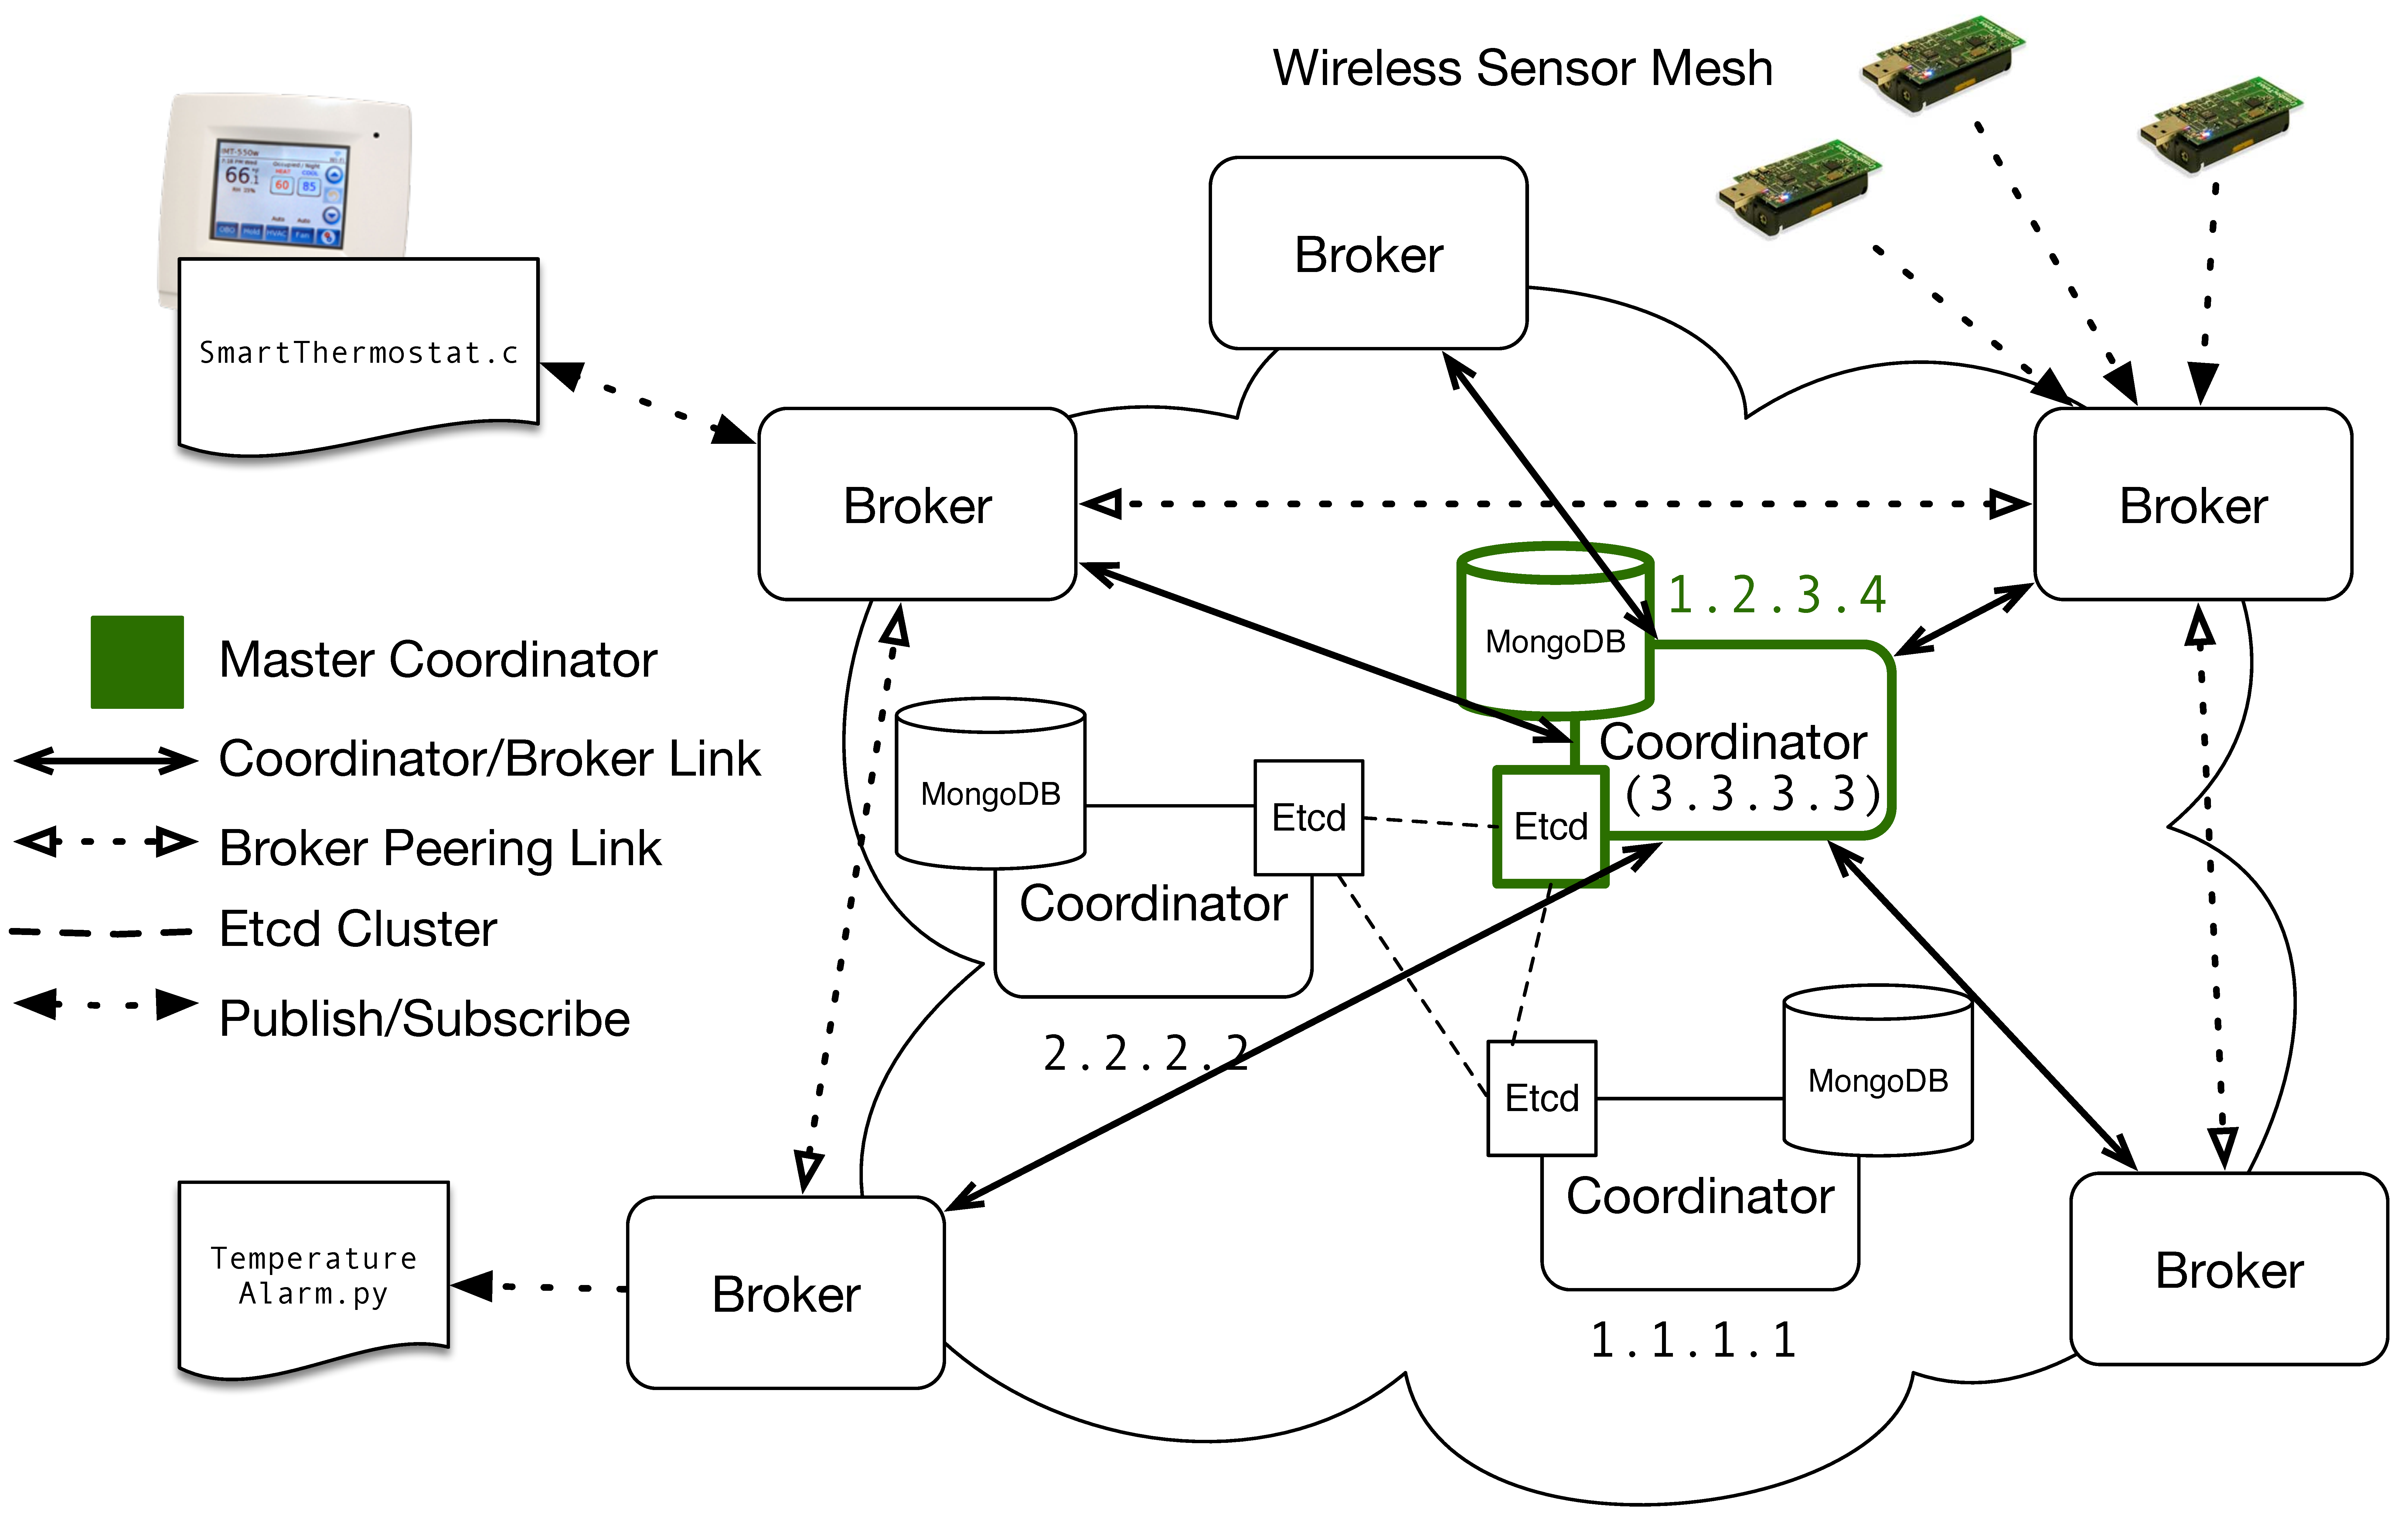
\includegraphics[width=6.5in]{figs/full_architecture.pdf}
\caption{Overview of the architecture of our brokerage system.
Numerous clients communicate to a set of decentralized brokers which create a forwarding network between themselves as instructed by the centralized coordinator nodes.}
\label{fig:architecture}
\end{figure*}

To meet these goals, we have developed an architecture which consists of two primary components: distributed brokers and centralized coordinators.
See Figure~\ref{fig:architecture} for an overview which will be described in more detail in this and the following sections.

The system contains one logically centralized coordinator; to all other entities in the system, the coordinator can be treated as a single machine.
In actuality, this logical coordinator consists of three independent nodes to improve fault tolerance; see Section~\ref{subsec:coordinator_fault_tolerance} for more detail.
This coordinator makes all of the decisions in the system, determining when a broker has failed, which brokers should forward which messages where, when changes occur to the set of publishers a subscriber is currently receiving messages from, which broker a client should contact if their broker fails, etc.
It then distributes these decisions to the brokers, which take appropriate action.
To do this the coordinator stores the current state of all brokers in the system, as well as information about all of the clients that are known to the system, i.e.\ what broker they are attached to, what query they are interested in (for subscribers), and what their current metadata is (for publishers).

Brokers are numerous and may reside anywhere; for example, a deployment may consist of a broker located in each building which contains client devices, or brokers may be run on cloud computing nodes.
Brokers are responsible for communicating with clients and for forwarding messages along routes as instructed by the coordinator.
Any changes to the set of clients connected to the broker, or to the metadata of a publisher connected to the broker, are communicated back to the coordinator for handling so that the coordinator always has an update-to-date view of the entire system state.

\subsection{Normal Operation}

In this section we describe the events which take place under normal operation, i.e.\ in the case that there are no failures within the system.

\textbf{A new subscriber submits a query.}
A subscriber contacts its local broker, whose address can be hardcoded into the client or discovered through some network discovery protocol, e.g.\ % TODO Gabe can you help here
The subscriber submits a message containing the query for which it is interested in receiving relevant messages.


\subsection{Broker Fault-Tolerance}

\subsection{Coordinator Fault-Tolerance}
\label{subsec:coordinator_fault_tolerance}

\subsection{Design Discussion}

% Evaluate design: simplicity of client protocol, etc. etc.

Note that this design creates a bottleneck at the coordinator, which must be contacted for all changes to the state of the system.
We assume that in comparison to the rate of messages being sent in the system, changes to the set of connected clients and to the metadata associated with publishers is relatively slow.
Since message forwarding can be done locally at a broker, distributing the brokers allows for high scalability in terms of number of messages that can be sent in the system, though if changes to the system state occur frequently enough the coordinator will become overloaded.
Part of the reason for choosing this design was its relative simplicity; we have two alternate designs discussed in Section~\ref{subsec:alternate_designs} which were considered and which we hope to evaluate as future work.


\subsection{Alternate Designs Considered}
\label{subsec:alternate_designs}
?
